% Problem 18: Dirichlet's Decay Factor
\begin{problem}[Dirichlet's Decay Factor: Taming $\sin^2 x$]

\textbf{Historical Context:}

In the 19th century, Peter Gustav Lejeune Dirichlet faced a stubborn puzzle: the integral 

$$\int_0^\infty \frac{\sin x}{x}\, dx$$

involves oscillations that never settle, yet the total area is finite. 
His key move was to introduce an exponential \emph{decay factor} $e^{-tx}$---multiplying a wild wave by something that fades with time forces the tail to die away, so a limit can exist.

\vspace{0.3cm}

The same idea appears far beyond the classroom. A car hitting a speed bump sets the suspension oscillating; without \textbf{damping}, those vibrations would persist indefinitely. A shock absorber dissipates energy, so each bounce is smaller than the last---exactly the role of $e^{-x}$ here. The wave $\sin^2 x$ keeps producing positive ``humps'' forever, but $e^{-x}$ acts as a mathematical shock absorber, bleeding away their contribution until only a finite total area remains.

\vspace{0.3cm}

Having seen how exponential decay tames an endless wave, apply the same idea to 
$$\int_0^\infty \frac{\sin^2 x}{e^x} \, dx$$

\vspace{0.3cm}
\textbf{Problem Statement:}

\textbf{(i)} Show that $f(x) = \frac{\sin^2 x}{e^x}$ can be written as:
$$f(x) = \frac{1}{2} e^{-x} - \frac{1}{2} e^{-x} \cos 2x$$

\textbf{(ii)} Use integration by parts to find 

$$\int e^{-x} \cos 2x \, dx$$

\textbf{(iii)} Hence, or otherwise, evaluate the improper integral:
$$\int_0^\infty \frac{\sin^2 x}{e^x} \, dx$$

\end{problem}

\begin{hint}
\begin{itemize}
    \item \textbf{Part (a):} Recall the double angle formula for $\cos 2x$. Make $\sin^2 x$ the subject and distribute $e^{-x}$.
    \item \textbf{Part (b):} Apply double integration by parts. Let $I = \int e^{-x} \cos 2x \, dx$. After two iterations, $I$ will reappear on the right-hand side. Solve algebraically for $I$.
    \item \textbf{Part (c):} Integrate the expression from (a) using your result from (b). As $x \to \infty$, remember that $e^{-x} \to 0$ while trigonometric functions remain strictly bounded.
\end{itemize}
\end{hint}

\begin{solution}
\textbf{Part (i)} \\
Using the double angle identity $\cos 2x = 1 - 2\sin^2 x$, rearrange for $\sin^2 x$:
$$\sin^2 x = \frac{1}{2}(1 - \cos 2x)$$
Substitute this into $f(x)$:
$$f(x) = e^{-x} \left( \frac{1 - \cos 2x}{2} \right) = \frac{1}{2} e^{-x} - \frac{1}{2} e^{-x} \cos 2x$$

\textbf{Part (ii)} \\
Let $I = \int e^{-x} \cos 2x \, dx$. \\
Apply integration by parts ($u = \cos 2x, dv = e^{-x}dx$):
$$I = -e^{-x} \cos 2x - 2 \int e^{-x} \sin 2x \, dx$$
Apply integration by parts again to the new integral ($u = \sin 2x, dv = e^{-x}dx$):
$$\int e^{-x} \sin 2x \, dx = -e^{-x} \sin 2x + 2 \int e^{-x} \cos 2x \, dx = -e^{-x} \sin 2x + 2I$$
Substitute this back into the equation for $I$:
$$I = -e^{-x} \cos 2x - 2(-e^{-x} \sin 2x + 2I)$$
$$I = -e^{-x} \cos 2x + 2e^{-x} \sin 2x - 4I$$
$$5I = e^{-x}(2\sin 2x - \cos 2x) \implies I = \frac{1}{5} e^{-x}(2\sin 2x - \cos 2x) + C$$

\textbf{Part (iii)} \\
Using the identity from (i) and the antiderivative from (ii):
$$\int_0^\infty \frac{\sin^2 x}{e^x} \, dx = \left[ -\frac{1}{2}e^{-x} - \frac{1}{10}e^{-x}(2\sin 2x - \cos 2x) \right]_0^\infty$$
Evaluate at the bounds $0$ and $\infty$: \\
\textbf{As $x \to \infty$:} $-\frac{1}{2}e^{-x} - \frac{1}{10}e^{-x}(2\sin 2x - \cos 2x) \to 0$ \\
\textbf{At $x = 0$:} $-\frac{1}{2}e^0 - \frac{1}{10}e^0(0 - 1) = -\frac{1}{2} + \frac{1}{10} = -\frac{2}{5}$ \\
Subtracting the lower bound from the upper bound gives:
$$= 0 - \left(-\frac{2}{5}\right) = \frac{2}{5}$$
\end{solution}

\begin{takeaways}
\begin{itemize}
    \item \textbf{The Power of Linearisation:} By converting $\sin^2 x$ into a linear $\cos 2x$ term, we sidestep an impossible integration and unlock the looping integration-by-parts method.
    \item \textbf{Generalisation ($e^{-ax} \sin bx$):} This strategy scales. Any integral in the form $\int_0^\infty e^{-ax} \sin^2(bx) \, dx$ or $\int_0^\infty e^{-ax} \cos(bx) \, dx$ can be solved using these exact same principles without altering the core logic.
    \item \textbf{Dirichlet's Taming Principle and the Laplace Transform:} Tame an endlessly repeating positive wave with exponential decay, then read off a finite area. This miniature version of Dirichlet's 19th-century idea reappears in damped harmonic motion, shock-absorber and vibration-control design, and the Laplace transform $\mathcal{L}\{f(x)\} = \int_0^\infty e^{-sx} f(x) \, dx$---solving this problem is exactly $\mathcal{L}\{\sin^2 x\}$ evaluated at $s=1$.
    \item \textbf{Complex Analysis Shortcut:} While HSC students must use integration by parts, uni math often evaluate these oscillating real-valued integrals elegantly in a single step using \textbf{Euler's Formula} ($e^{i\theta} = \cos \theta + i\sin \theta$) or \textbf{Cauchy's Residue Theorem}.
\end{itemize}
\end{takeaways}

\begin{remark}[Normanhurst Boys High School Trial 2024, Ext 2 Q 16(b)]
If you like this style of problem, try Normanhurst Boys High School Trial 2024 Extension~2 Question~16(b) below:

\medskip

The diagram shows a sketch of part of the curve with equation
$$ y = e^{-x} \sin x \quad x \ge 0 $$

\begin{center}
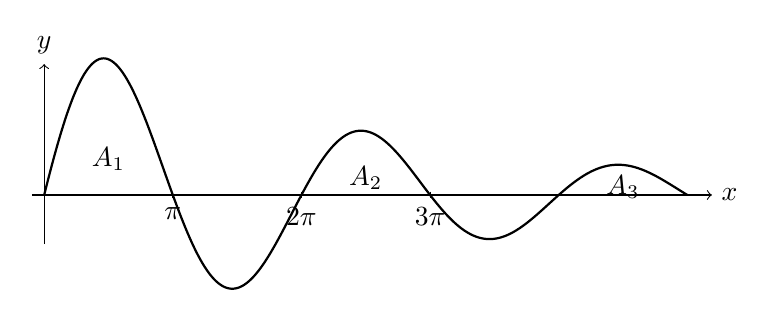
\begin{tikzpicture}[scale=0.52]
    % Axes (extended to show three positive humps: $A_1$, $A_2$, $A_3$)
    \draw[->] (-0.3,0) -- ({5*pi + 0.6},0) node[right] {$x$};
    \draw[->] (0,-1.2) -- (0,3.2) node[above] {$y$};

    % Curve: scaled sketch of $y = e^{-x}\sin x$ for visual clarity
    \draw[thick, domain=0:{5*pi}, samples=400, smooth]
        plot (\x, {4*exp(-0.12*\x)*sin(\x*180/pi)});

    % Ticks and labels at $\pi$, $2\pi$, $3\pi$
    \draw ({pi},0.08) -- ({pi},-0.08) node[below] {$\pi$};
    \draw ({2*pi},0.08) -- ({2*pi},-0.08) node[below] {$2\pi$};
    \draw ({3*pi},0.08) -- ({3*pi},-0.08) node[below] {$3\pi$};

    % Area labels on successive positive humps
    \node at ({0.5*pi}, {1.05*exp(-0.12*0.5*pi)}) {$A_1$};
    \node at ({2.5*pi}, {1.05*exp(-0.12*2.5*pi)}) {$A_2$};
    \node at ({4.5*pi}, {1.05*exp(-0.12*4.5*pi)}) {$A_3$};
\end{tikzpicture}
\end{center}

\begin{enumerate}[label=(\roman*)]
    \item Show that
    $$ \int e^{-x} \sin x \, dx = -\frac{1}{2} e^{-x} (\sin x + \cos x) + C $$

    \item The terms $A_1, A_2, \cdots, A_n$ represent successive areas above the $x$-axis and bounded by the curve $y = e^{-x} \sin x$.

    The area $A_n$ is bounded by the curve $y = e^{-x} \sin x$ between $x = (2n - 2)\pi$ and $x = (2n - 1)\pi$.

    The areas represented by $A_1$ and $A_2$ are shown in the diagram.

    Show that
    $$ A_n = \frac{1}{2} \left( e^{(1-2n)\pi} + e^{(2-2n)\pi} \right) $$

    \item Show that
    $$ A_1 + A_2 + A_3 + \cdots $$
    is a geometric series, and has $\displaystyle \frac{e^\pi}{2(e^\pi - 1)}$ as its limiting sum.

    \item Given that $\displaystyle \lim_{n \to \infty} \int_0^n e^{-x} \sin x \, dx = \frac{1}{2}$, find the exact value of
    $$ \lim_{n \to \infty} \int_0^n \left| e^{-x} \sin x \right| dx $$
\end{enumerate}
\end{remark}

\begin{remark}[A cleaner route to part (iv)]
To avoid the pain of $|{\sin x}|$ and geometric series, there is a clean shortcut. Let
\[
I = \int_0^\infty e^{-x} \left| \sin x \right| dx.
\]
Split at $x = \pi$:
\[
I = \int_0^\pi e^{-x} \left| \sin x \right| dx + \int_\pi^\infty e^{-x} \left| \sin x \right| dx.
\]
Substitute $u = x - \pi$ in the second integral:
\[
\int_\pi^\infty e^{-x} \left| \sin x \right| dx
= \int_0^\infty e^{-(u+\pi)} \left| \sin(u+\pi) \right| du
= e^{-\pi} \int_0^\infty e^{-u} \left| \sin u \right| du
= e^{-\pi} I.
\]
On $[0,\pi]$, $\sin x \ge 0$, so $\left| \sin x \right| = \sin x$. Hence
\[
I = \int_0^\pi e^{-x} \sin x \, dx + e^{-\pi} I.
\]

Apply double-integration by parts to $\int e^{-x} \sin x \, dx$ to find its value, then rearrange to express $I$ in terms of this integral, which can be refferenced from part (i).
\end{remark}
